
% \subsection{The Sensinact edge gateway}
% The communication between sensors/actuators and the Edge is facilitated by a gateway. An edge gateway, also referred to as an edge device, is a network device that functions as the entry point for data traffic between diverse networks. In addition to routing and protocol conversion, the edge gateway fulfills various functions. It plays a crucial role in enabling the seamless data flow between networks while ensuring connectivity and interoperability. Typically, the edge gateway is deployed at the network's edge, serving mainly as protocol conversion. In the work context, we depend on the Sensinact gateway, which has been brought to fruition after a series of European projects, namely BigClouT \cite{ref144}, WISE IoT \cite{ref145}, IoF2020 \cite{ref146}, ActivAge \cite{ref147}, and ultimately Brain-IoT \cite{brainiot2022}. The specificity of the Sensinact gateway lies in its ability to enable designers and edge architects to specify the data flow using the Sensinact language. The \fig{sensinact} portrays the internal structure of the Sensinact gateway composed of northbound and southbound bridges. The \textit{northbound} bridge provides crucial functionalities for interfacing with remote servers using costly protocols such as HTTP/HTTPS. It supports a wide range of protocols, such as HTTP REST, MQTT, XMPP, JSON RPC, and CDMI.  The \textit{southbound} module facilitates the interaction with sensors and actuators, utilizing various device protocols such as Zigbee, LoRa, and MQTT. In this paper, we will not address the details related to the gateway as they are available in the Brain-IoT deliverables. We would to enhance the southbound bridges of the gateway by supporting RabbiotMQ protocol \cite{Rabbitmq}. The difference from southbound bridge protocols, such as MQTT, lies in its support for asynchronous messages through  message queuing.


This section presents the formalization of the RabbitMQ Architecture to make it compatible with the Concurrent Stochastic Game (CSG). We also provide a formal implementation of RabbitMQ in PRISM games. We formalize and model the CAPEC-384 \cite{capec384} attack at various protocol levels, specifically focusing on data corruption, and establish semantic rules to capture their impact.



\subsection{The RabbitMQ architecture}
%In \fig{rabbitarchitecture}, we illustrate the architecture of RabbitMQ, which consists of a set of sensors (Producers) and one actuator (consumer). A Raspberry Pi serves as a connectivity interface that converts signals into data sensitive to attacks and acts as both a consumer and producer. The exchange is responsible for accepting messages from the producers and routing them to message queues based on \textbf{binding key}. For example, the water level queue is associated with the binding key \emph{binding key = wl\_pl}. The exchange examines the message properties derived from the sensor's message to extract the \textbf{routing key}, a virtual address used to determine which message queue the message will be stored in by matching the binding keys. 

%\BH{Update the figure with the FOG and the Gateway explicitley}

In \fig{fig:rabbitarchitecture}, we present the architectural depiction of RabbitMQ deployed on an IoT gateway. This deployment comprises a set of Producers, specifically three sensors: water level (WL), water volume (WV), and rain precipitation (RP), as well as two consumers, including one actuator and the Fog. Additionally, a connectivity interface is incorporated to convert signals into data, which is susceptible to attacks, and it serves both the consumers and producers. The exchange is designed to accept messages from the producers and direct them to message queues based on a designated \textbf{binding key}. For instance, the water level queue is associated with the binding key \emph{binding key = wl\_pl}. The exchange scrutinizes the message properties derived from the producers' messages in order to extract the \textbf{routing key}, which functions as a virtual address that determines the appropriate message queue for storage by matching the binding keys. Formally, a RabbitMQ system during execution is defined as follows:

\begin{mydef} \label{def:rq} \normalfont (RabbitMQ). A RabbitMQ system \quot{\emath{\mathcal{RQ}}} is a tuple \emath{\mathcal{RQ}= \langle \mathcal{M}, RK, BK, E, Q\rangle}, where: 
 \begin{itemize}
\item \emath{\mathcal{M}} is the message structure alive in \emath{\mathcal{RQ}}, 
\item \emath{RK}= \emath{\{ rk_{0}, \ldots,rk_{n} \} } is a set of routing keys,
\item \emath{BK}= \emath{ \{ bk_{0}, \ldots,bk_{n}  \} } is a set of binding keys,
\item \emath{E} is the exchange node of the system, and 
\item \emath{Q} = \emath{\{ q_{0}, \ldots, q_{n}\}} is a set of queues supported by \emath{\mathcal{RQ}}. 
            \end{itemize}
\end{mydef}


Throughout the paper, we consider a message composed of a \emph{routing key and a payload}. Formally, we define a RabbitMQ message as:

\begin{mydef} \label{def:message} \normalfont (Message). A RabbitMQ message \quot{\emath{\mathcal{M}}} is a tuple \emath{\mathcal{M}= \langle rk, pld\rangle}, where: 
 \begin{itemize}
\item \emath{rk} is the routing key of sensors message and
\item \emath{pld} is the payload of the sensed data
            \end{itemize}
\end{mydef}
\begin{figure}[!htb]
           
\noindent
     \centering

		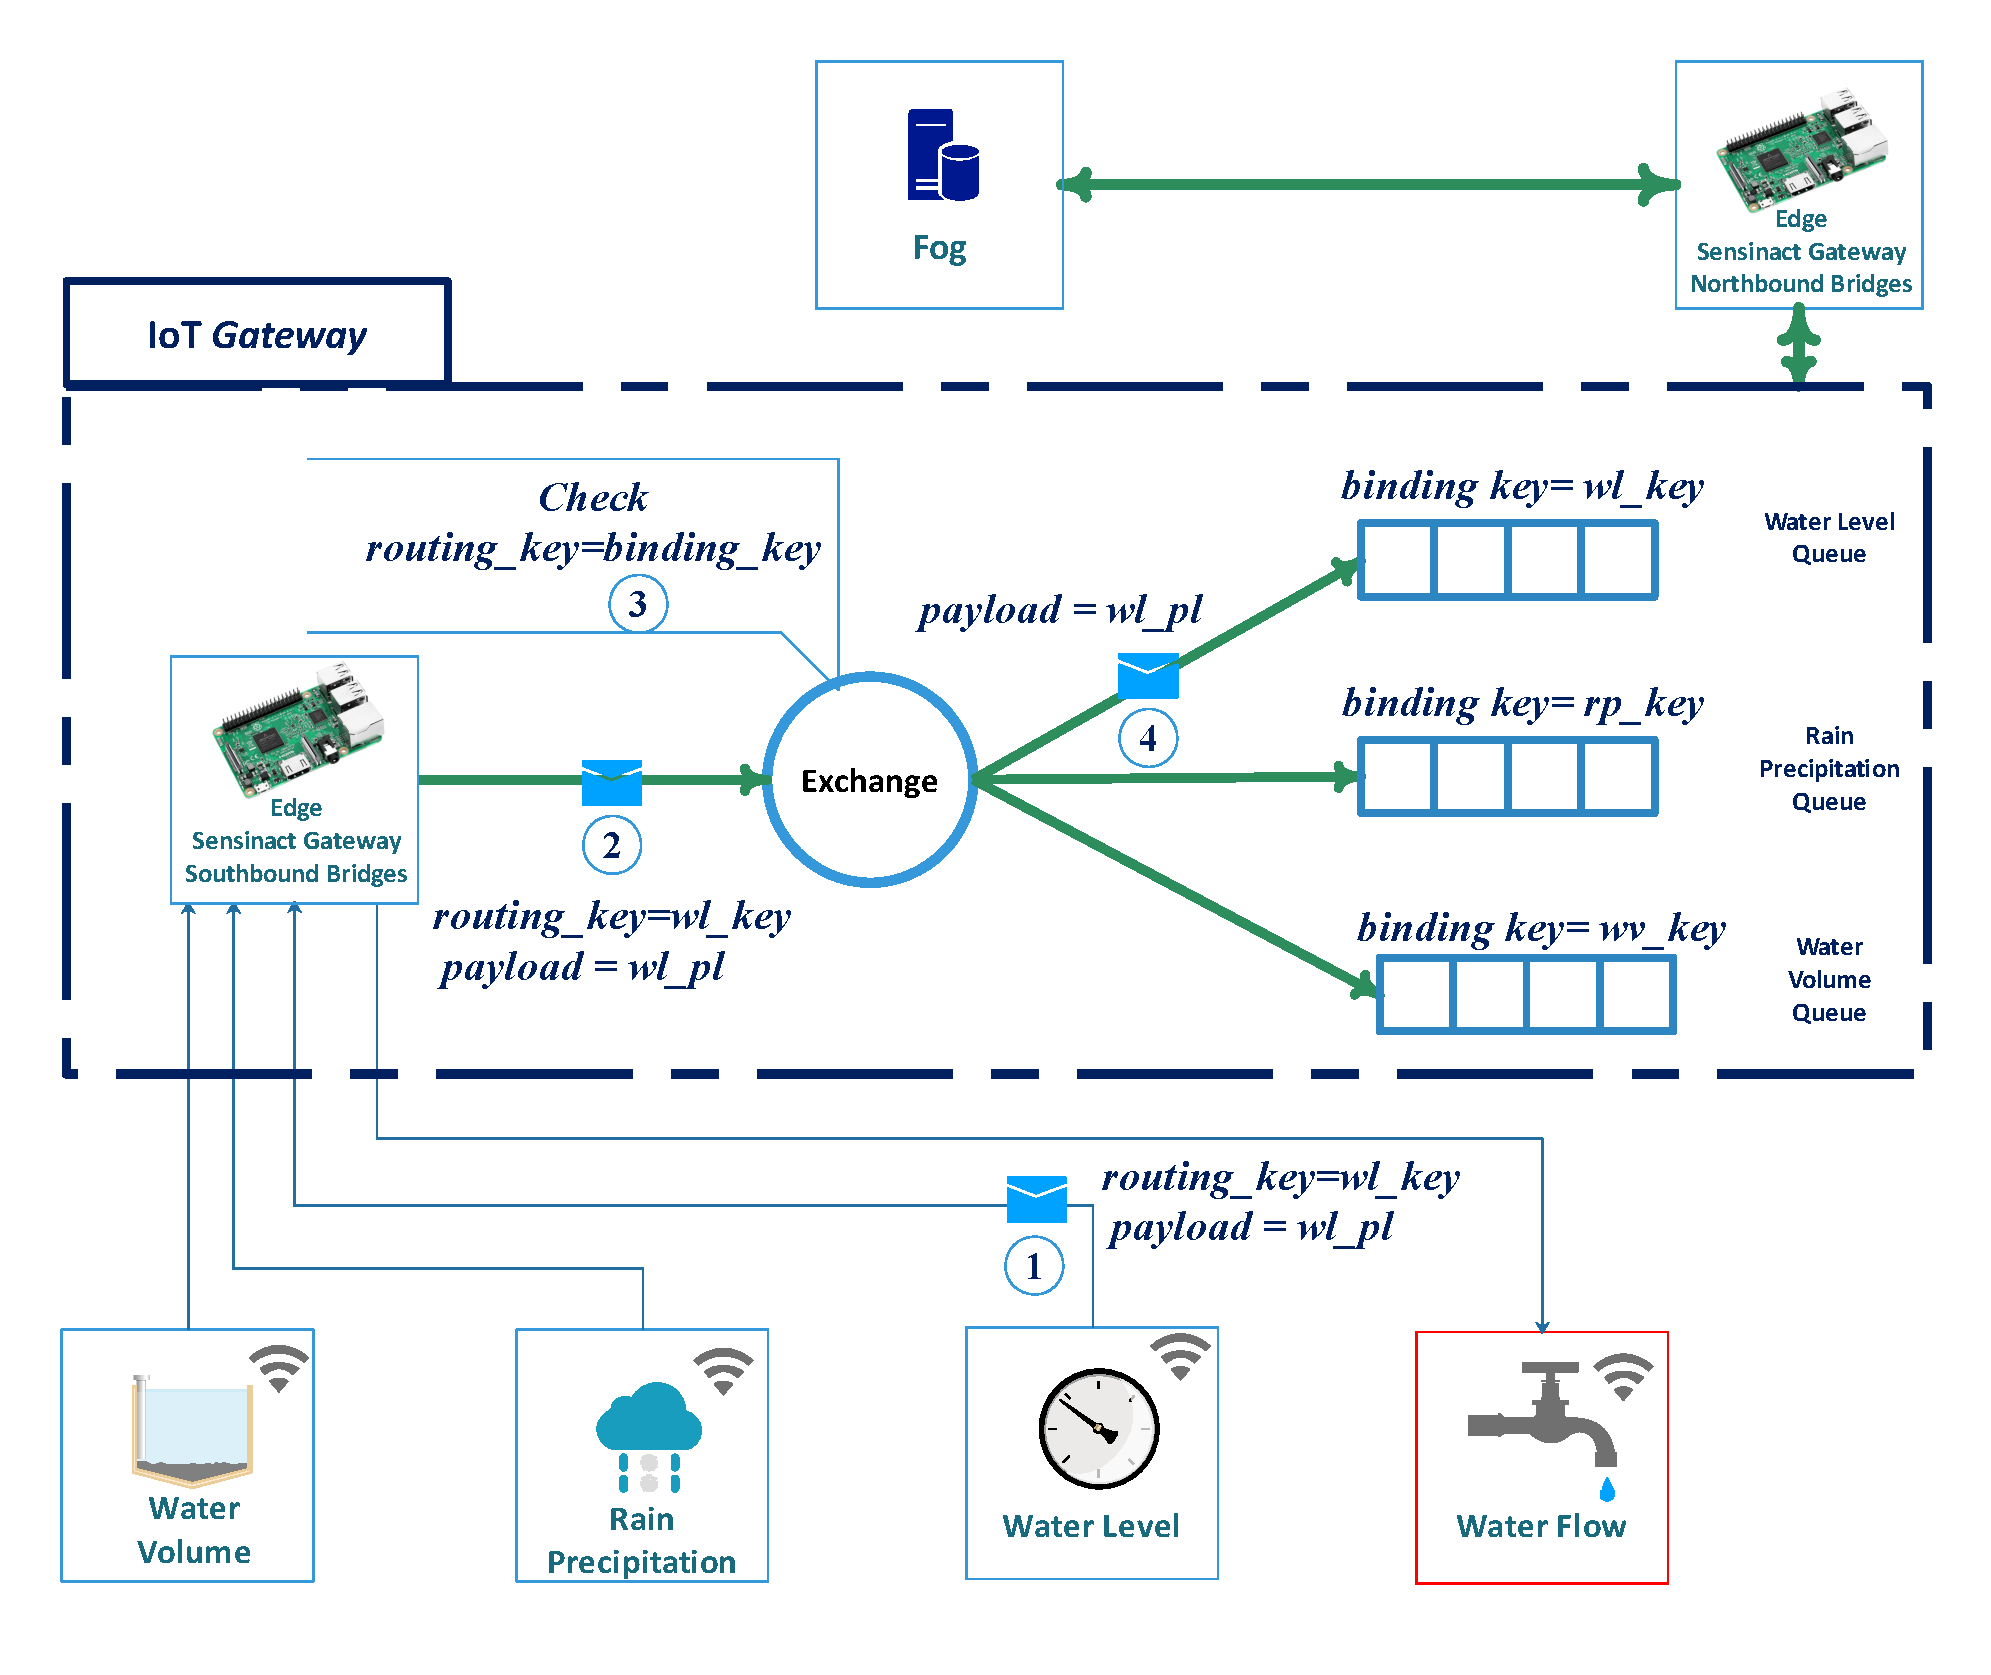
\includegraphics[width=263pt, height =200pt]{ArchitectureRabbit.pdf}
		\caption{The RabbitMQ Architecture for IoT.}
	\label{fig:rabbitarchitecture}
\end{figure}

\subsection{Communication formalism for RabbitMQ architecture in PRISM-games}
%\BH{missing D3!!}
In the PRISM-games formalism, the modeling of communication and resource access is facilitated through the use of player and non-player modules. Players are distinguished by unique action labels, while non-CSG players are identified by multiple action labels. For instance, each component of the modeled system in \fig{fig:rabbitarchitecture} is considered as a PRISM module where reading and writing is enabled by access to local PRISM module variables.


%In the PRISM module, \emath{rk} and \emath{pld} are local variables initialized to queue keys and sensed data, respectively. Each component of the modeled system in \fig{fig:rabbitarchitecture} is considered as a PRISM module where reading is enabled to other PRISM models with the PRISM system.


The algebraic expression of the message \emath{m} transmitted from module \emath{\mathcal{D}_{1}} to \emath{\mathcal{D}_{2}} is expressed through channeling \cite{baierprinciples2008} using send (!) and receive (?) symbols as : \emath{\sset{\mathcal{D}_{s}}=l_{1} \gparrow{\langle a!m \rangle} l_{2}} saying that  \emath{\mathcal{D}_{s}} transmit the message through the channel \emath{a} (PRISM action) and \emath{\sset{\mathcal{D}_{r}}=l_{3} \gparrow{\langle a?x \rangle}l_{4}} saying that \emath{a?x} receives a message via channel \emath{a} and assign it to variable \emath{x}.


However, building upon the player definition provided in the previous section, we introduce a two-player rule that involves a competition based on writing. \emath{\mathcal{D}_{3}} records the messages received from both players \emath{\mathcal{D}_{1}} and \emath{\mathcal{D}_{2}.}The rule \ref{writing} is defined as follows:

\begin{boxD}
%\framedtext{
	      \begin{equation}\frac{\sset{\mathcal{D}_{1}}= l_{1}\gparrow{a!m_{1}}l'_{1} \wedge \sset{\mathcal{D}_{2}}= l_{2}\gparrow{b!m_{2} }l'_{2}  \wedge
        \sset{\mathcal{D}_{3}}= l_{3}\gparrow{a?k_{1}, b?k_{2}}l'_{3}        
       } {  \langle l_{1},\ldots,l_{2},\ldots l_{3},\theta\rangle  \xrightarrow{a,b}\langle l'_{1},\ldots,l'_{2},\ldots,l'_{3},\theta'\rangle } \tag{\emph{Writing}} \label{writing} \end{equation} where \emath{\theta':=\theta[ k_{1}:= m_{1}, k_2:=m_{2}]} and \emath{\mathcal{D}_{1}, \mathcal{D}_{2}} are two CSG players.
%}

\end{boxD}


\subsection{Queues modeling}
\label{sec:threats:manif}

The RabbitMQ queues are responsible for storing the sensed data based on the routing key present in the transmitted messages. The Exchange module verifies the correspondence between the routing key and the binding key in order to carry out the operation. Firstly, the \emath{Queue} module is regarded as a player responsible for data storage. It is characterized by the queue variable and the identifier binding key, as depicted in lines 1-3 of the code snippet of \lst{queueemodel}. As the PRISM language lacks native support for the list data type, it is necessary to define the list cases and the index variable, as mentioned in lines 1-2. To traverse the queue, we require an item index that is initialized to 0 at line 5. 
\noindent
\begin{figure}[!htb]
    \centering
    

\tikzset{every picture/.style={line width=1.05pt}} %set default line width to 0.75pt        

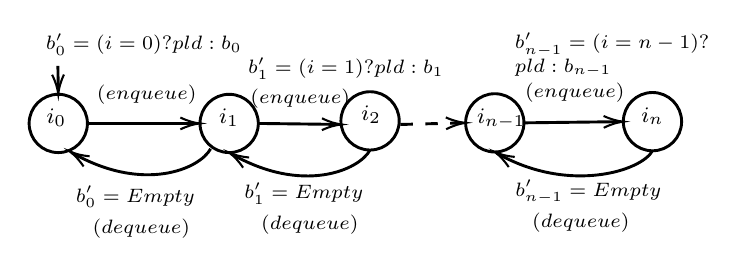
\begin{tikzpicture}[x=0.65pt,y=0.65pt,yscale=-1,xscale=1]
%uncomment if require: \path (0,300); %set diagram left start at 0, and has height of 300


%Shape: Circle [id:dp31914676096119765] 
\draw   (74.6,98.1) .. controls (74.6,89.15) and (81.85,81.9) .. (90.8,81.9) .. controls (99.75,81.9) and (107,89.15) .. (107,98.1) .. controls (107,107.05) and (99.75,114.3) .. (90.8,114.3) .. controls (81.85,114.3) and (74.6,107.05) .. (74.6,98.1) -- cycle ;
%Straight Lines [id:da37317958939159324] 
\draw    (90.6,66.13) -- (90.78,79.9) ;
\draw [shift={(90.8,81.9)}, rotate = 269.29] [color={rgb, 255:red, 0; green, 0; blue, 0 }  ][line width=0.75]    (10.93,-3.29) .. controls (6.95,-1.4) and (3.31,-0.3) .. (0,0) .. controls (3.31,0.3) and (6.95,1.4) .. (10.93,3.29)   ;
%Shape: Circle [id:dp22901745321019074] 
\draw   (169.6,98.1) .. controls (169.6,89.15) and (176.85,81.9) .. (185.8,81.9) .. controls (194.75,81.9) and (202,89.15) .. (202,98.1) .. controls (202,107.05) and (194.75,114.3) .. (185.8,114.3) .. controls (176.85,114.3) and (169.6,107.05) .. (169.6,98.1) -- cycle ;
%Shape: Circle [id:dp6850049335985016] 
\draw   (317.27,97.77) .. controls (317.27,88.82) and (324.52,81.57) .. (333.47,81.57) .. controls (342.41,81.57) and (349.67,88.82) .. (349.67,97.77) .. controls (349.67,106.71) and (342.41,113.97) .. (333.47,113.97) .. controls (324.52,113.97) and (317.27,106.71) .. (317.27,97.77) -- cycle ;
%Straight Lines [id:da10806683009608209] 
\draw    (107,98.1) -- (167.6,98.1) ;
\draw [shift={(169.6,98.1)}, rotate = 180] [color={rgb, 255:red, 0; green, 0; blue, 0 }  ][line width=0.75]    (10.93,-3.29) .. controls (6.95,-1.4) and (3.31,-0.3) .. (0,0) .. controls (3.31,0.3) and (6.95,1.4) .. (10.93,3.29)   ;
%Straight Lines [id:da8217014567182165] 
\draw  [dash pattern={on 4.5pt off 4.5pt}]  (281,98.67) -- (315.27,97.82) ;
\draw [shift={(317.27,97.77)}, rotate = 178.58] [color={rgb, 255:red, 0; green, 0; blue, 0 }  ][line width=0.75]    (10.93,-3.29) .. controls (6.95,-1.4) and (3.31,-0.3) .. (0,0) .. controls (3.31,0.3) and (6.95,1.4) .. (10.93,3.29)   ;
%Shape: Circle [id:dp08560151992011589] 
\draw   (247.93,96.67) .. controls (247.93,87.72) and (255.19,80.47) .. (264.13,80.47) .. controls (273.08,80.47) and (280.33,87.72) .. (280.33,96.67) .. controls (280.33,105.61) and (273.08,112.87) .. (264.13,112.87) .. controls (255.19,112.87) and (247.93,105.61) .. (247.93,96.67) -- cycle ;
%Straight Lines [id:da7410245959347421] 
\draw    (202,98.1) -- (246.33,98.64) ;
\draw [shift={(248.33,98.67)}, rotate = 180.7] [color={rgb, 255:red, 0; green, 0; blue, 0 }  ][line width=0.75]    (10.93,-3.29) .. controls (6.95,-1.4) and (3.31,-0.3) .. (0,0) .. controls (3.31,0.3) and (6.95,1.4) .. (10.93,3.29)   ;
%Shape: Circle [id:dp4984227004498517] 
\draw   (404.93,97.1) .. controls (404.93,88.15) and (412.19,80.9) .. (421.13,80.9) .. controls (430.08,80.9) and (437.33,88.15) .. (437.33,97.1) .. controls (437.33,106.05) and (430.08,113.3) .. (421.13,113.3) .. controls (412.19,113.3) and (404.93,106.05) .. (404.93,97.1) -- cycle ;
%Straight Lines [id:da9002692791455889] 
\draw    (349.67,97.77) -- (402.93,97.12) ;
\draw [shift={(404.93,97.1)}, rotate = 179.31] [color={rgb, 255:red, 0; green, 0; blue, 0 }  ][line width=0.75]    (10.93,-3.29) .. controls (6.95,-1.4) and (3.31,-0.3) .. (0,0) .. controls (3.31,0.3) and (6.95,1.4) .. (10.93,3.29)   ;
%Curve Lines [id:da054067545547898055] 
\draw    (421.13,113.3) .. controls (415.06,124.55) and (374.49,137.41) .. (334.67,114.67) ;
\draw [shift={(333.47,113.97)}, rotate = 30.52] [color={rgb, 255:red, 0; green, 0; blue, 0 }  ][line width=0.75]    (10.93,-3.29) .. controls (6.95,-1.4) and (3.31,-0.3) .. (0,0) .. controls (3.31,0.3) and (6.95,1.4) .. (10.93,3.29)   ;
%Curve Lines [id:da19389154071839954] 
\draw    (264.13,112.87) .. controls (258.06,124.12) and (226.64,137.72) .. (187,115) ;
\draw [shift={(185.8,114.3)}, rotate = 30.52] [color={rgb, 255:red, 0; green, 0; blue, 0 }  ][line width=0.75]    (10.93,-3.29) .. controls (6.95,-1.4) and (3.31,-0.3) .. (0,0) .. controls (3.31,0.3) and (6.95,1.4) .. (10.93,3.29)   ;
%Curve Lines [id:da5969865187078301] 
\draw    (175.47,112.2) .. controls (169.39,123.45) and (137.97,137.06) .. (98.34,114.33) ;
\draw [shift={(97.13,113.63)}, rotate = 30.52] [color={rgb, 255:red, 0; green, 0; blue, 0 }  ][line width=0.75]    (10.93,-3.29) .. controls (6.95,-1.4) and (3.31,-0.3) .. (0,0) .. controls (3.31,0.3) and (6.95,1.4) .. (10.93,3.29)   ;


% Text Node
\draw (108,149) node [anchor=north west][inner sep=0.75pt]  [font=\scriptsize]  {$( dequeue)$};
% Text Node
\draw (98.67,131) node [anchor=north west][inner sep=0.75pt]  [font=\scriptsize]  {$b_{0} '=Empty$};
% Text Node
\draw (201.67,147) node [anchor=north west][inner sep=0.75pt]  [font=\scriptsize]  {$( dequeue)$};
% Text Node
\draw (192.33,129) node [anchor=north west][inner sep=0.75pt]  [font=\scriptsize]  {$b_{1} '=Empty$};
% Text Node
\draw (352.33,145.67) node [anchor=north west][inner sep=0.75pt]  [font=\scriptsize]  {$( dequeue)$};
% Text Node
\draw (348.33,73.67) node [anchor=north west][inner sep=0.75pt]  [font=\scriptsize]  {$( enqueue)$};
% Text Node
\draw (335,45.67) node [anchor=north west][inner sep=0.75pt]  [font=\scriptsize]  {$ \begin{array}{l}
b_{n-1} '=( i=n-1) ?\\
pld:b_{n-1}
\end{array}$};
% Text Node
\draw (413,87.33) node [anchor=north west][inner sep=0.75pt]  [font=\footnotesize]  {$i_{n}$};
% Text Node
\draw (257.33,86.33) node [anchor=north west][inner sep=0.75pt]  [font=\footnotesize]  {$i_{2}$};
% Text Node
\draw (343,127.67) node [anchor=north west][inner sep=0.75pt]  [font=\scriptsize]  {$b_{n-1} '=Empty$};
% Text Node
\draw (195.67,77) node [anchor=north west][inner sep=0.75pt]  [font=\scriptsize]  {$( enqueue)$};
% Text Node
\draw (194.33,59.67) node [anchor=north west][inner sep=0.75pt]  [font=\scriptsize]  {$b_{1} '=( i=1) ?pld:b_{1}$};
% Text Node
\draw (82,46.33) node [anchor=north west][inner sep=0.75pt]  [font=\scriptsize]  {$b_{0} '=( i=0) ?pld:b_{0}$};
% Text Node
\draw (110.33,74.67) node [anchor=north west][inner sep=0.75pt]  [font=\scriptsize]  {$( enqueue)$};
% Text Node
\draw (321.67,88) node [anchor=north west][inner sep=0.75pt]  [font=\footnotesize]  {$i_{n-1}$};
% Text Node
\draw (178.33,88) node [anchor=north west][inner sep=0.75pt]  [font=\footnotesize]  {$i_{1}$};
% Text Node
\draw (82.33,88) node [anchor=north west][inner sep=0.75pt]  [font=\footnotesize]  {$i_{0}$};


\end{tikzpicture}
    \caption{Queue Model.}
    \label{fig:queue}
\end{figure} 

To enhance clarity, the enqueue and dequeue operations are modeled as automata in \fig{fig:queue}. At each state (corresponding to an index value), the \emph{enqueue} operation is performed, and the variables \emath{b_{0},\ldots,b_{1}} are assigned the value of the payload, denoted as $pld$ following the rule \ref{writing}. The consumer (for example a Fog) executes the dequeue operation, while a non-player module stores the dequeued data that will be consumed. The command in line 6 executes the automata model depicted in \fig{fig:queue}, where each state represents an index value. Additionally, we utilize a conditional structure in command line 6 to assign the value of $pld$ to the corresponding variable $b_{i}$ based on the index value. In the dequeue operation, the synchronization based on the dequeue channel is carried out with the command in line 9.

\lstdefinestyle{framed}
{
	frame=lrb,         
	mathescape,
	numbers=left,
	belowcaptionskip=-1pt,
    xleftmargin=3em,
		xrightmargin=0.01cm,
    framexleftmargin=3em,
	framexrightmargin=0pt,
	framextopmargin=5pt,
	framexbottommargin=5pt,
	framesep=0pt,
	rulesep=0pt,
	numbers=left,
}
    
\lstset{
    breaklines=true,
    style=framed,
    escapeinside={<@}{@>},
    morekeywords={void, int, public, private, class, protected, submodules, network, connections, const, init, int, bool, double, module, rewards, endrewards, endmodule},
    basicstyle=\ttfamily,
    keywordstyle=\bfseries\color{blue},
        morecomment=[f][\color{green!30!black}][0]{/*},
    morecomment=[l][\color{green!30!black}]{//},
    label=queueemodel
}



\begin{figure}[!htb]            
\begin{minipage}{16cm}
\begin{lstlisting}[style=framed,%customc,
	caption=PRISM Code for the Queue Player,
 	label=queueemodel]	
module Queue
 $b_{0}$: [INIT_VAL..MAX_VAL]  init EMPTY;
 $b_{1}$: [INIT_VAL..MAX_VAL]  init EMPTY;
 $bk$ : [KEY_0..KEY_0] init KEY_0;
 i   :[0..QUEUE_MAX] init 0;
 [enqueue] i<QUEUE_MAX -> (i'=mod(i+1,QUEUE_MAX))  &($b_{0}$'=(i=0)?$pld_{3}$:$b_{0}$) &($b_{1}$'=(i=1)?$pld_{3}$:$b_{1}$);
 [dequeue] i>0 -> (i'=i-1)  &($b_{0}$'=(i=0)?EMPTY:$b_{0}$)  &($b_{1}$'=(i=1)?EMPTY:$b_{1}$); 
endmodule
\end{lstlisting}
 \end{minipage}  
\end{figure}

The model, consisting of one producer (sensor), one queue, and one consumer (fog), can be accessed through the following link: \cite{edcc23} under reference \texttt{M2}. In the following section, we instantiate multiple queues and sensors to facilitate the exchange of messages through a use case.



\subsection{Attacks modeling}
\label{sec:threats:manif}

In this section, we formalize the attack CAPEC-384 \cite{capec384} that can impact the messages exchanged between communicating entities, thereby affecting both the payload and the routing key. For each message $m$ we use the following notations:  $rk$ denotes the routing key of the message $m$, $rk_{x}$ denotes the erroneous routing key of the message $m$, $pld$ denotes the payload of the message $m$, and $pld_{x}$ denotes the erroneous payload of the message $m$.

\emph{Tampering} \cite{shostack2014threat}  leads to the alteration of messages transmitted by the sender component through the communication port. Within the context of \emath{\mathcal{RQ}} system, ${pld}$ is altered during the message transfer. Considering the sensor player \emath{\mathcal{D}_{1}} and attacker player \emath{\mathcal{D}_{2}} where the exchange node manages the interaction modeled as \emath{\mathcal{D}_{3}}. When refining the rule (\ref{writing}), the outcomes of routing key tampering are expressed through rules \ref{rkSuccess} and \ref{rkFailure}. Specifically, rule \ref{rkSuccess} represents the successful tampering of the routing key, while rule \ref{rkFailure} represents the failure to tamper with the routing key.

%\BH{refer in the text to \emph{rk Success} and \emph{rk Failure}}

\begin{boxD}
%\framedtext{
	      \begin{equation}\label{rkSuccess} \frac{ \sset{\mathcal{D}_{1}}= l_{1}\gparrow{a!\gl{rk_{1},pld_{1}}}l'_{1} \wedge \sset{\mathcal{D}_{2}}= l_{2}\gparrow{b!\gl{rk_{x},pld_{2}} }l'_{2} \wedge
         \sset{\mathcal{D}_{3}}= l_{3}\gparrow{a, b?\gl{rk_{3},pld_{3}}}_{p}l'_{3}       
       } {  \langle l_{1},\ldots,l_{2},\ldots l_{3},\theta\rangle  \xrightarrow{a,b}_{p}\langle l'_{1},\ldots,l'_{2},\ldots,l'_{3},\theta'\rangle } \tag{\emph{rk Success}} \end{equation} where \emath{\theta':=\theta[rk_{3}=rk_{x},pld_{3}=pld_{2}]} and \emath{\mathcal{D}_{1}} is the sensor, \emath{\mathcal{D}_{2}} is the attacker. \emath{p} is the success rate of the attacker.

	      \begin{equation}\label{rkFailure}\frac{ \sset{\mathcal{D}_{1}}= l_{1}\gparrow{a!\gl{rk_{1},pld_{1}}}l'_{1} \wedge \sset{\mathcal{D}_{2}}=  l_{2}\gparrow{b!\gl{rk_{x},pld_{2}} }l'_{2} \wedge
         \sset{\mathcal{D}_{3}}= l_{3}\gparrow{a, b?\gl{rk_{3},pld_{3}}}_{1-p}l'_{3}       
       } {  \langle l_{1},\ldots,l_{2},\ldots l_{3},\theta\rangle  \xrightarrow{a,b}_{1-p}\langle l'_{1},\ldots,l'_{2},\ldots,l'_{3},\theta'\rangle } \tag{\emph{rk Failure}} \end{equation} where \emath{\theta':=\theta[rk_{3}=rk_{1},pld_{3}=pld_{1}]} and \emath{\mathcal{D}_{1}} is the sensor, \emath{\mathcal{D}_{2}} is the attacker. \emath{1-p} is the failure rate of the attacker.
\end{boxD}


Since the model incorporates the stochastic behavior of the system, it accurately represents the success and failure of the attacker using a stochastic parameter \emath{p}. 

% Add a reference to the learning frequencies algorithm presented in section ***

This parameter enables us to effectively model the message loss of the sensor at the exchange level as a result of the attack. While we address the issue of routing key tampering, it is also necessary to model payload tampering caused by similar attacks. Then, the success and failure rules are expressed by the rules \ref{pld Success} and \ref{pld Failure}.


\begin{boxD}
%\framedtext{
	      \begin{equation}\frac{ \sset{\mathcal{D}_{1}}= l_{1}\gparrow{a!\gl{rk_{1},pld_{1}}}l'_{1} \wedge \sset{\mathcal{D}_{2}}=  l_{2}\gparrow{b!\gl{rk_{2},pld_{x}} }l'_{2} \wedge
        \sset{\mathcal{D}_{3}}=  l_{3}\gparrow{a, b?\gl{rk_{3},pld_{3}}}_{p}l'_{3}      
       } {  \langle l_{1},\ldots,l_{2},\ldots l_{3},\theta\rangle  \xrightarrow{a,b}_{p}\langle l'_{1},\ldots,l'_{2},\ldots,l'_{3},\theta'\rangle } \label{pld Success} \tag{\emph{pld Success}} \end{equation} where \emath{\theta':=\theta[rk_{3}=rk_{1},pld_{3}=pld_{x}]} and \emath{\mathcal{D}_{1}} is the sensor, \emath{\mathcal{D}_{2}} is the attacker. \emath{p} is the success rate of the attacker.
%}
	      \begin{equation}\frac{\sset{\mathcal{D}_{1}}= l_{1}\gparrow{a!\gl{rk_{1},pld_{1}}}l'_{1} \wedge \sset{\mathcal{D}_{2}}= l_{2}\gparrow{b!\gl{rk_{2},pld_{x}} }l'_{2} \wedge
        \sset{\mathcal{D}_{3}}=  l_{3}\gparrow{a, b?\gl{rk_{3},pld_{3}}}_{1-p}l'_{3}       
       } {  \langle l_{1},\ldots,l_{2},\ldots l_{3},\theta\rangle  \xrightarrow{a,b}_{1-p}\langle l'_{1},\ldots,l'_{2},\ldots,l'_{3},\theta'\rangle } \label{pld Failure}  \tag{\emph{pld Failure}} \end{equation} where \emath{\theta':=\theta[rk_{3}=rk_{1},pld_{3}=pld_{1}]} and \emath{\mathcal{D}_{1}} is the sensor, \emath{\mathcal{D}_{2}} is the attacker. \emath{1-p} is the failure rate of the attacker.
\end{boxD}

Now, with the formal specification of attacks at the exchange, we can proceed to provide a projection onto the PRISM code. Before modeling the exchange module of the interaction system, we present in \fig{fig:attack:sensor} the attacker and producer players model. They are characterized by two channels (we employ the terminology used for the channeling system \cite{baierprinciples2008}): write and wait. The write channel is responsible for transmitting the produced value from the producer (i.e., attacker) to the exchange node. The writing and waiting operations are performed each round \emath{r}. 

\noindent
\begin{figure}[!htb]
    \centering
    


\tikzset{every picture/.style={line width=1.05pt}} %set default line width to 0.75pt        

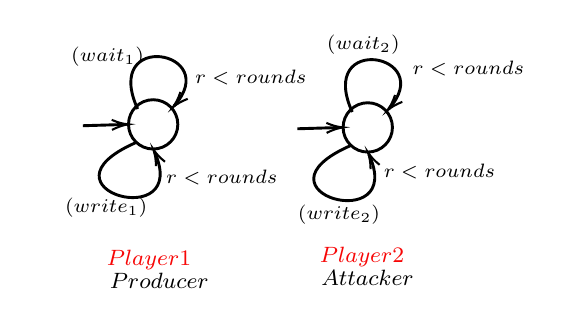
\begin{tikzpicture}[x=0.55pt,y=0.55pt,yscale=-1,xscale=1]
%uncomment if require: \path (0,300); %set diagram left start at 0, and has height of 300

%Shape: Circle [id:dp760252948462048] 
\draw   (192.6,79.1) .. controls (192.6,70.15) and (199.85,62.9) .. (208.8,62.9) .. controls (217.75,62.9) and (225,70.15) .. (225,79.1) .. controls (225,88.05) and (217.75,95.3) .. (208.8,95.3) .. controls (199.85,95.3) and (192.6,88.05) .. (192.6,79.1) -- cycle ;
%Curve Lines [id:da3741641705012937] 
\draw    (198.6,69) .. controls (174.84,16.53) and (254.97,30.71) .. (222.62,66.9) ;
\draw [shift={(221.6,68)}, rotate = 313.41] [color={rgb, 255:red, 0; green, 0; blue, 0 }  ][line width=0.75]    (10.93,-3.29) .. controls (6.95,-1.4) and (3.31,-0.3) .. (0,0) .. controls (3.31,0.3) and (6.95,1.4) .. (10.93,3.29)   ;
%Curve Lines [id:da7883550885112647] 
\draw    (197.6,91) .. controls (127.31,121.69) and (234.42,151.4) .. (209.59,96.98) ;
\draw [shift={(208.8,95.3)}, rotate = 63.88] [color={rgb, 255:red, 0; green, 0; blue, 0 }  ][line width=0.75]    (10.93,-3.29) .. controls (6.95,-1.4) and (3.31,-0.3) .. (0,0) .. controls (3.31,0.3) and (6.95,1.4) .. (10.93,3.29)   ;
%Straight Lines [id:da8536170630459327] 
\draw    (162.6,80) -- (190.6,79.16) ;
\draw [shift={(192.6,79.1)}, rotate = 178.28] [color={rgb, 255:red, 0; green, 0; blue, 0 }  ][line width=0.75]    (10.93,-3.29) .. controls (6.95,-1.4) and (3.31,-0.3) .. (0,0) .. controls (3.31,0.3) and (6.95,1.4) .. (10.93,3.29)   ;
%Shape: Circle [id:dp7766834825103327] 
\draw   (51.6,77.1) .. controls (51.6,68.15) and (58.85,60.9) .. (67.8,60.9) .. controls (76.75,60.9) and (84,68.15) .. (84,77.1) .. controls (84,86.05) and (76.75,93.3) .. (67.8,93.3) .. controls (58.85,93.3) and (51.6,86.05) .. (51.6,77.1) -- cycle ;
%Curve Lines [id:da6262481144264533] 
\draw    (57.6,67) .. controls (33.84,14.53) and (113.97,28.71) .. (81.62,64.9) ;
\draw [shift={(80.6,66)}, rotate = 313.41] [color={rgb, 255:red, 0; green, 0; blue, 0 }  ][line width=0.75]    (10.93,-3.29) .. controls (6.95,-1.4) and (3.31,-0.3) .. (0,0) .. controls (3.31,0.3) and (6.95,1.4) .. (10.93,3.29)   ;
%Curve Lines [id:da4372707429069086] 
\draw    (56.6,89) .. controls (-13.69,119.69) and (93.42,149.4) .. (68.59,94.98) ;
\draw [shift={(67.8,93.3)}, rotate = 63.88] [color={rgb, 255:red, 0; green, 0; blue, 0 }  ][line width=0.75]    (10.93,-3.29) .. controls (6.95,-1.4) and (3.31,-0.3) .. (0,0) .. controls (3.31,0.3) and (6.95,1.4) .. (10.93,3.29)   ;
%Straight Lines [id:da6134143403844121] 
\draw    (21.6,78) -- (49.6,77.16) ;
\draw [shift={(51.6,77.1)}, rotate = 178.28] [color={rgb, 255:red, 0; green, 0; blue, 0 }  ][line width=0.75]    (10.93,-3.29) .. controls (6.95,-1.4) and (3.31,-0.3) .. (0,0) .. controls (3.31,0.3) and (6.95,1.4) .. (10.93,3.29)   ;

% Text Node
\draw (179.6,16) node [anchor=north west][inner sep=0.75pt]  [font=\scriptsize]  {$( wait_{2})$};
% Text Node
\draw (176,170.3) node [anchor=north west][inner sep=0.75pt]  [font=\footnotesize]  {$Attacker$};
% Text Node
\draw (175,155.3) node [anchor=north west][inner sep=0.75pt]  [font=\footnotesize,color={rgb, 255:red, 247; green, 6; blue, 6 }  ,opacity=1 ]  {$Player2$};
% Text Node
\draw (7.6,123) node [anchor=north west][inner sep=0.75pt]  [font=\scriptsize]  {$( write_{1})$};
% Text Node
\draw (11.6,24) node [anchor=north west][inner sep=0.75pt]  [font=\scriptsize]  {$( wait_{1})$};
% Text Node
\draw (37,172.3) node [anchor=north west][inner sep=0.75pt]  [font=\footnotesize]  {$Producer$};
% Text Node
\draw (35,157.3) node [anchor=north west][inner sep=0.75pt]  [font=\footnotesize,color={rgb, 255:red, 247; green, 6; blue, 6 }  ,opacity=1 ]  {$Player1$};
% Text Node
\draw (160.6,128) node [anchor=north west][inner sep=0.75pt]  [font=\scriptsize]  {$( write_{2})$};
% Text Node
\draw (236,33) node [anchor=north west][inner sep=0.75pt]  [font=\scriptsize]  {$r< rounds\ $};
% Text Node
\draw (217,101) node [anchor=north west][inner sep=0.75pt]  [font=\scriptsize]  {$r< rounds\ $};
% Text Node
\draw (93,39) node [anchor=north west][inner sep=0.75pt]  [font=\scriptsize]  {$r< rounds\ $};
% Text Node
\draw (74,105) node [anchor=north west][inner sep=0.75pt]  [font=\scriptsize]  {$r< rounds\ $};


\end{tikzpicture}

    \caption{Attacker and Sensor Models.}
    \label{fig:attack:sensor}
\end{figure} 


The exchange system captures the interactions between producers (sensors) and attackers in the \lst{exchangemodel}, specifically focusing on the payload transfer. This is achieved through the utilization of two channels, namely $write_{1}$ and $write_{2}$. The success and failure rules, denoted as \ref{pld Success} and \ref{pld Failure}, are implemented through the PRISM commands found in lines 4-5. Additionally, players have the ability to enter a waiting mode, which is modeled using two channels, $wait_{1}$ and $wait_{2}$, implemented as actions in PRISM. In the case of waiting modes, the exchange module resets both internal binding keys and payload in line 6. However, if one of the players is available to transfer its payload, a non-probabilistic command is implemented in lines 7-8.

\lstdefinestyle{framed}
{
	frame=lrb,         
	mathescape,
	numbers=left,
	belowcaptionskip=-1pt,
    xleftmargin=3em,
		xrightmargin=0.01cm,
    framexleftmargin=3em,
	framexrightmargin=0pt,
	framextopmargin=5pt,
	framexbottommargin=5pt,
	framesep=0pt,
	rulesep=0pt,
	numbers=left,
}
\lstset{
    breaklines=true,
    style=framed,
    escapeinside={<@}{@>},
    morekeywords={void, int, public, private, class, protected, submodules, network, connections, const, init, int, bool, double, module, rewards, endrewards, endmodule},
    basicstyle=\ttfamily,
    keywordstyle=\bfseries\color{blue},
        morecomment=[f][\color{green!30!black}][0]{/*},
    morecomment=[l][\color{green!30!black}]{//},
    label=queueemodel
}



\begin{figure}[!htb]            
\begin{minipage}{16.5cm}
\begin{lstlisting}[style=framed,%customc,
	caption=PRISM code for Exchange Module,
 	label=exchangemodel]	
module Exchange
$pld_{3}$  : [INIT_VAL..MAX_VAL] init EMPTY;
$rk_{3}$ : [INIT_VAL..MAX_VAL] init EMPTY;
[$write_{1}$, $write_{2}$] true  -> (1-$p$):($pld_{3}$'=$pld_{1}$)&($rk_{3}$'=$rk_{3}$)  +$p$:($pld_{3}$'=$pld_{2}$)&($rk_{3}$'=$rk_{2}$);
[$wait_{1}$ , $wait_{2}$]  true -> ($pld_{3}$'=EMPTY) & ($rk_{3}$'=EMPTY);
[$write_{1}$, $wait_{2}$ ]  true -> ($pld_{3}$'=$pld_{1}$) &  ($rk_{3}$'=$rk_{1}$ );
[$wait_{1}$ , $write_{2}$]  true -> ($pld_{3}$'=$pld_{x}$) &  ($rk_{3}$'=$rk_{2}$ );
endmodule
\end{lstlisting}
 \end{minipage}  
\end{figure}

\paragraph*{Remark}The definition of binding key tampering follows the same principle as payload tampering.

